\begin{figure}[t]
  \scalebox{0.92}{
    \begin{tabular}{m{1pt}c@{\hspace{10pt}}c@{\hspace{10pt}}c}
      &\hspace{7pt}\small model: \labelcref{item:many-neuron-model}; data: $\texttt{Kur}(10)$) &
      \hspace{7pt}\small model: \labelcref{item:many-neuron-model}; data: $\texttt{Kur}(4)$ &
      \hspace{7pt}\small model: ICA; data: $\texttt{Kur}(3)$ \\
      \raisebox{62pt}{\rotatebox{90}{\tiny magnitude $w_i$}} &
      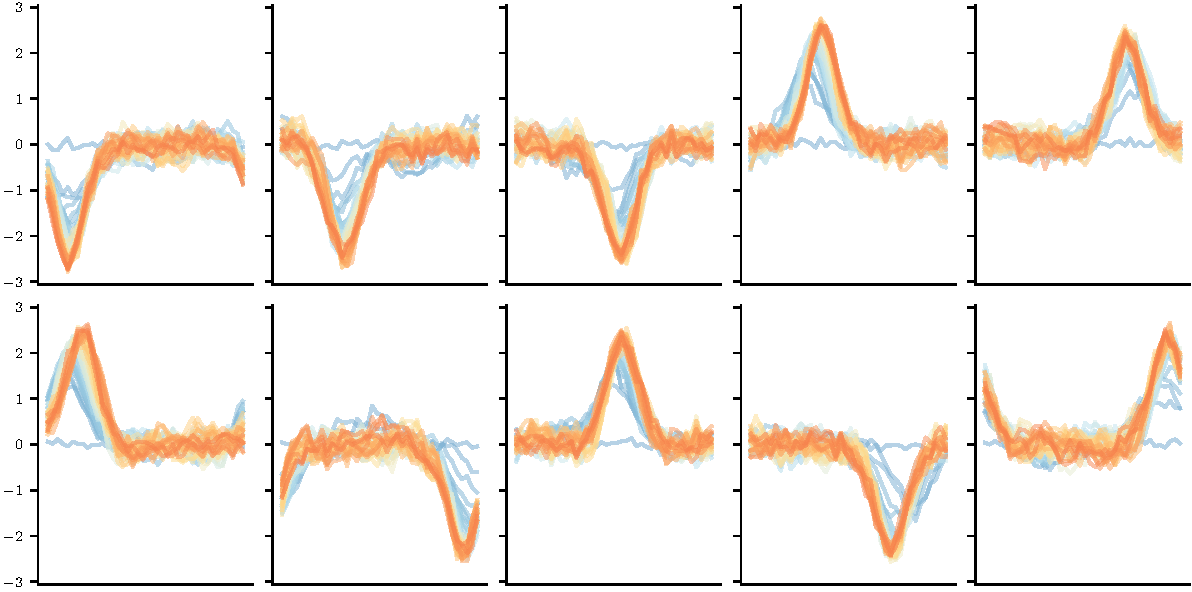
\includegraphics[width=0.33\linewidth]{figures/extensions/10erf_alg10.pdf} &
      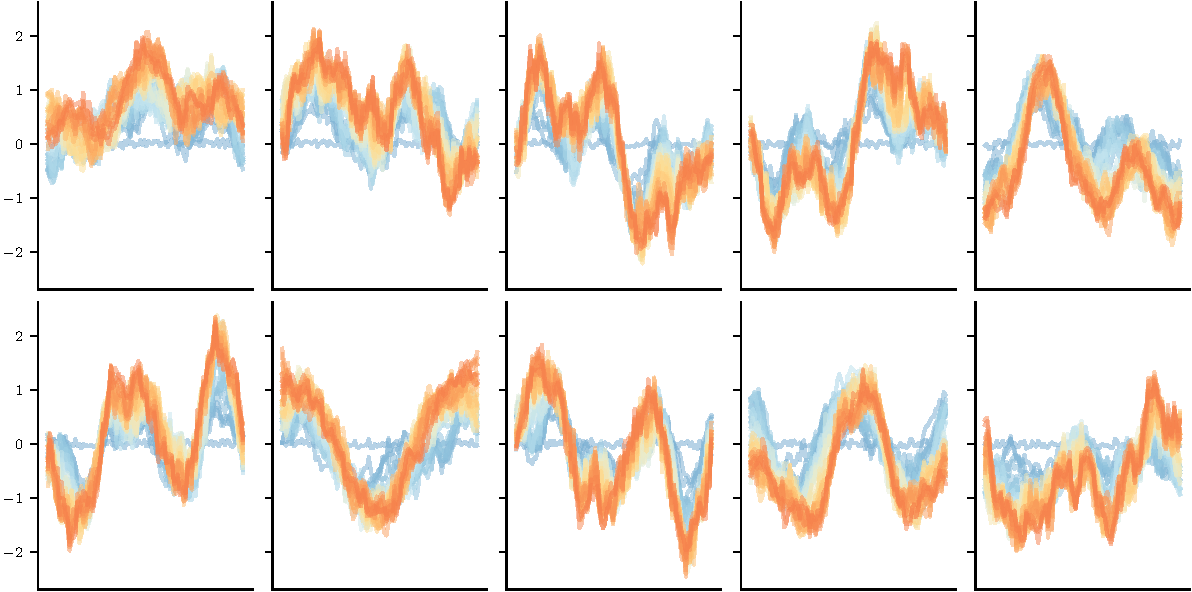
\includegraphics[width=0.33\linewidth]{figures/extensions/10erf_alg4.pdf} &
      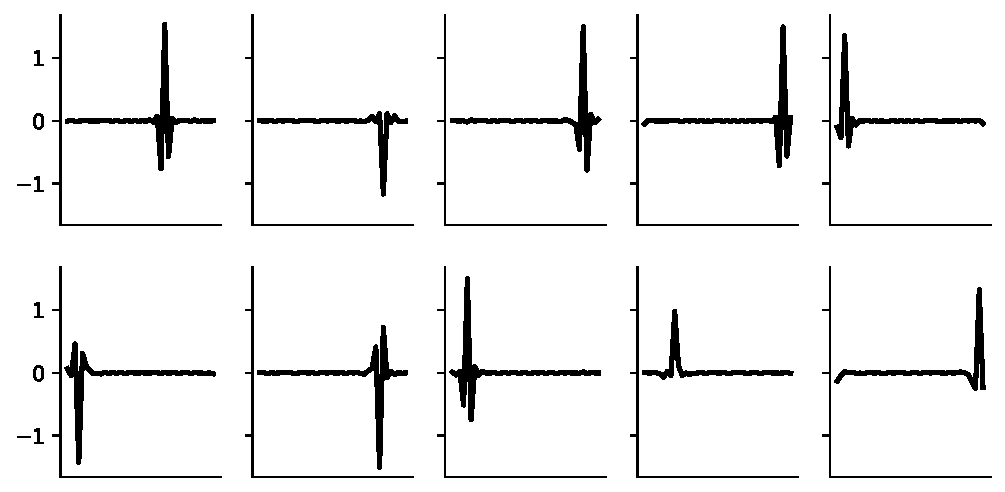
\includegraphics[width=0.33\linewidth]
      {figures/extensions/ica_alg3.pdf} \\
    \noalign{\vskip -48pt}
      &\hspace{7pt}\tiny dimension $i$ of weight $\mathbf{w}$ &
      \hspace{7pt}\tiny dimension $i$ of weight $\mathbf{w}$ &
    \hspace{7pt}\tiny dimension $i$ of weight $\mathbf{w}$ 
    \end{tabular}
  }
  \caption{
    (\textbf{Left}, \textbf{Center}) Receptive fields learned 
    by many-neuron (\labelcref{item:many-neuron-model}) 
    soft committee machines (second-layer weights fixed at $\frac{1}{K}$) 
    trained on the $\texttt{Kur}(10)$ and $\texttt{Kur}(4)$ datasets, respectively.
    The models had $N=40$ input units, $K=10$ hidden units, and an initialization variance of $0.1$.
    (\textbf{Right}) A random subset of 10 components from the 40 learned by 
    the FastICA algorithm from scikit-learn~\parencite{hyvarinen1999fast,scikit-learn} on the 
    $\texttt{Kur}(3)$ dataset with 
    length-scale correlation values of $\xi_0 = 1$ and $\xi_1 = 3$. 
    \emph{See \cref{sec:extensions} for exposition.}
  }
  \label{fig:extensions}
\end{figure}
